\documentclass[9pt, xcolor=table]{beamer}
%
% Packages
\usepackage[english]{babel} % Set language
\usepackage[T1]{fontenc}  % font Encoder for westeuropean languages
\usepackage[utf8]{inputenc} % Utf8 input encoder
\usepackage[autostyle=true,german=quotes]{csquotes} % quotation package
\usepackage[ddmmyyyy]{datetime} % for date and time formats
\usepackage[sorting=none,backend=bibtex8]{biblatex}  % bibliography package
\usepackage{pgfpages} % print multiple pages per slide
\usepackage[font={footnotesize}]{caption} %caption package
\usepackage{listings} % for code frame
\usepackage{xcolor} % color package
\usepackage{graphicx} % for images
\usepackage{float} % for float package
\usepackage{subfigure}
\usepackage{hyperref} 
\usepackage{amsmath,amssymb,amsthm}
\usepackage{newtxmath} % must come after amsXXX
%\usepackage{ziffer} % set , as decimal and . as thousand seperator (needed for german)
%
%
% activate to show notes on second screen:
%\setbeameroption{show notes on second screen}
%
%
% Bibliography
\addbibresource{references.bib} 
%
% Image Path
\graphicspath{{Images/}}
\DeclareGraphicsExtensions{.pdf, .jpg, .tif, .png, .gif}   
%
% Style
% Define style
\usetheme{Boadilla}
\useoutertheme{miniframes}
\useinnertheme{rectangles}

% Define colours
\definecolor{THblack}{HTML}{000000}
\definecolor{THRed}{RGB}{201,12,15}
\definecolor{THOrange}{RGB}{234,91,12}
\definecolor{THPurple}{RGB}{184,37,133}
\definecolor{BlueSaphirre}{HTML}{0B4F6C}
\definecolor{DartmouthGreen}{HTML}{306B34}
\def\cmd#1{\texttt{\color{red}\footnotesize $\backslash$#1}}
\def\env#1{\texttt{\color{blue}\footnotesize #1}}
\definecolor{deepblue}{rgb}{0,0,0.5}
\definecolor{deepred}{rgb}{0.6,0,0}
\definecolor{deepgreen}{rgb}{0,0.5,0}
\definecolor{halfgray}{gray}{0.55}


% define element colors
\setbeamercolor{palette primary}{bg=THPurple,fg=white}
\setbeamercolor{palette secondary}{bg=THRed,fg=white}
\setbeamercolor{palette tertiary}{bg=THOrange,fg=white}
\setbeamercolor{palette quaternary}{bg=THblack,fg=white}
\setbeamercolor{structure}{fg=THblack}
\setbeamercolor{title}{fg=THRed}
\setbeamercolor{frametitle}{fg=THOrange}
\setbeamercolor{mini frame}{fg=white, bg=THOrange}
\setbeamercolor{section in head/foot}{fg=white, bg=THOrange}
\setbeamercolor{structure}{fg=THblack}

% define Block colors
\setbeamercolor{block title}{bg=BlueSaphirre!50, fg=white}
\setbeamercolor{block body}{bg=BlueSaphirre!15}
\setbeamercolor{block title alerted}{bg=THRed!50, fg=white}
\setbeamercolor{block body alerted}{bg=THRed!15}
\setbeamercolor{block title example}{bg=DartmouthGreen!55, fg=white}
\setbeamercolor{block body example}{bg=DartmouthGreen!15}

% define element styles
\setbeamertemplate{headline}{}
\setbeamertemplate{section in toc shaded}[default][50]
\setbeamertemplate{section in toc}[square]
\setbeamertemplate{subsection in toc}[square]
\setbeamertemplate{itemize items}[square]
\setbeamertemplate{enumerate items}[square]
\setbeamertemplate{caption}[numbered]
\setbeamertemplate{blocks}[default]

% Show numbers instead of symbols in bibliography
\setbeamertemplate{bibliography item}{\insertbiblabel}
\renewcommand*{\bibfont}{\small} % make font smaller

%The next block of commands puts the table of contents at the 
%beginning of each section and highlights the current section:
\AtBeginSection[]{
	\begin{frame}{Contents}
		\tableofcontents[currentsection, hideallsubsections]
	\end{frame}
}

\AtBeginSubsection[]{
	\begin{frame}{Contents}
		\tableofcontents[sectionstyle=show/shaded,subsectionstyle=show/shaded/hide,subsubsectionstyle=hide]
	\end{frame}
}

\AtBeginSubsubsection[]{
	\begin{frame}{Contents}
		\tableofcontents[sectionstyle=show/shaded,subsectionstyle=show/shaded/hide,subsubsectionstyle=show/shaded/hide]
	\end{frame}
}

% restyle captions
\DeclareCaptionFont{grey}{\color{black!70}}
\captionsetup{
  labelfont={grey},
  textfont={grey}
}

%
%listings Style
\lstset{
	numbers=left,
	numberstyle= \small\color{halfgray}, 
    basicstyle=\ttfamily\small,
    keywordstyle=\bfseries\color{deepblue},
    emphstyle=\ttfamily\color{deepred},    % Custom highlighting style
    stringstyle=\color{deepgreen},
    rulesepcolor=\color{red!20!green!20!blue!20},
    % frame=shadowbox,
	breaklines=true
}
%
%Caption Style
\captionsetup[figure]{labelfont={bf},
                      labelformat={default},
                      labelsep=period,name={Figure}
                      }
\captionsetup[table]{labelfont={bf},
                      labelformat={default},
                      labelsep=period,name={Table}
                      }

%
% Title page information
\title[PyCG] {PyCG: Practical Call Graph Generation in Python}
\author[HE PEILIN]{HE PEILIN}
\institute[MUST] {2021 IEEE/ACM 43rd International Conference on Software Engineering (ICSE)\cite{9402076}}
\newcommand{\Contactmail}{\url{timhh991022@gmail.com}}
\date{\today}
%
% define title graphic
\titlegraphic {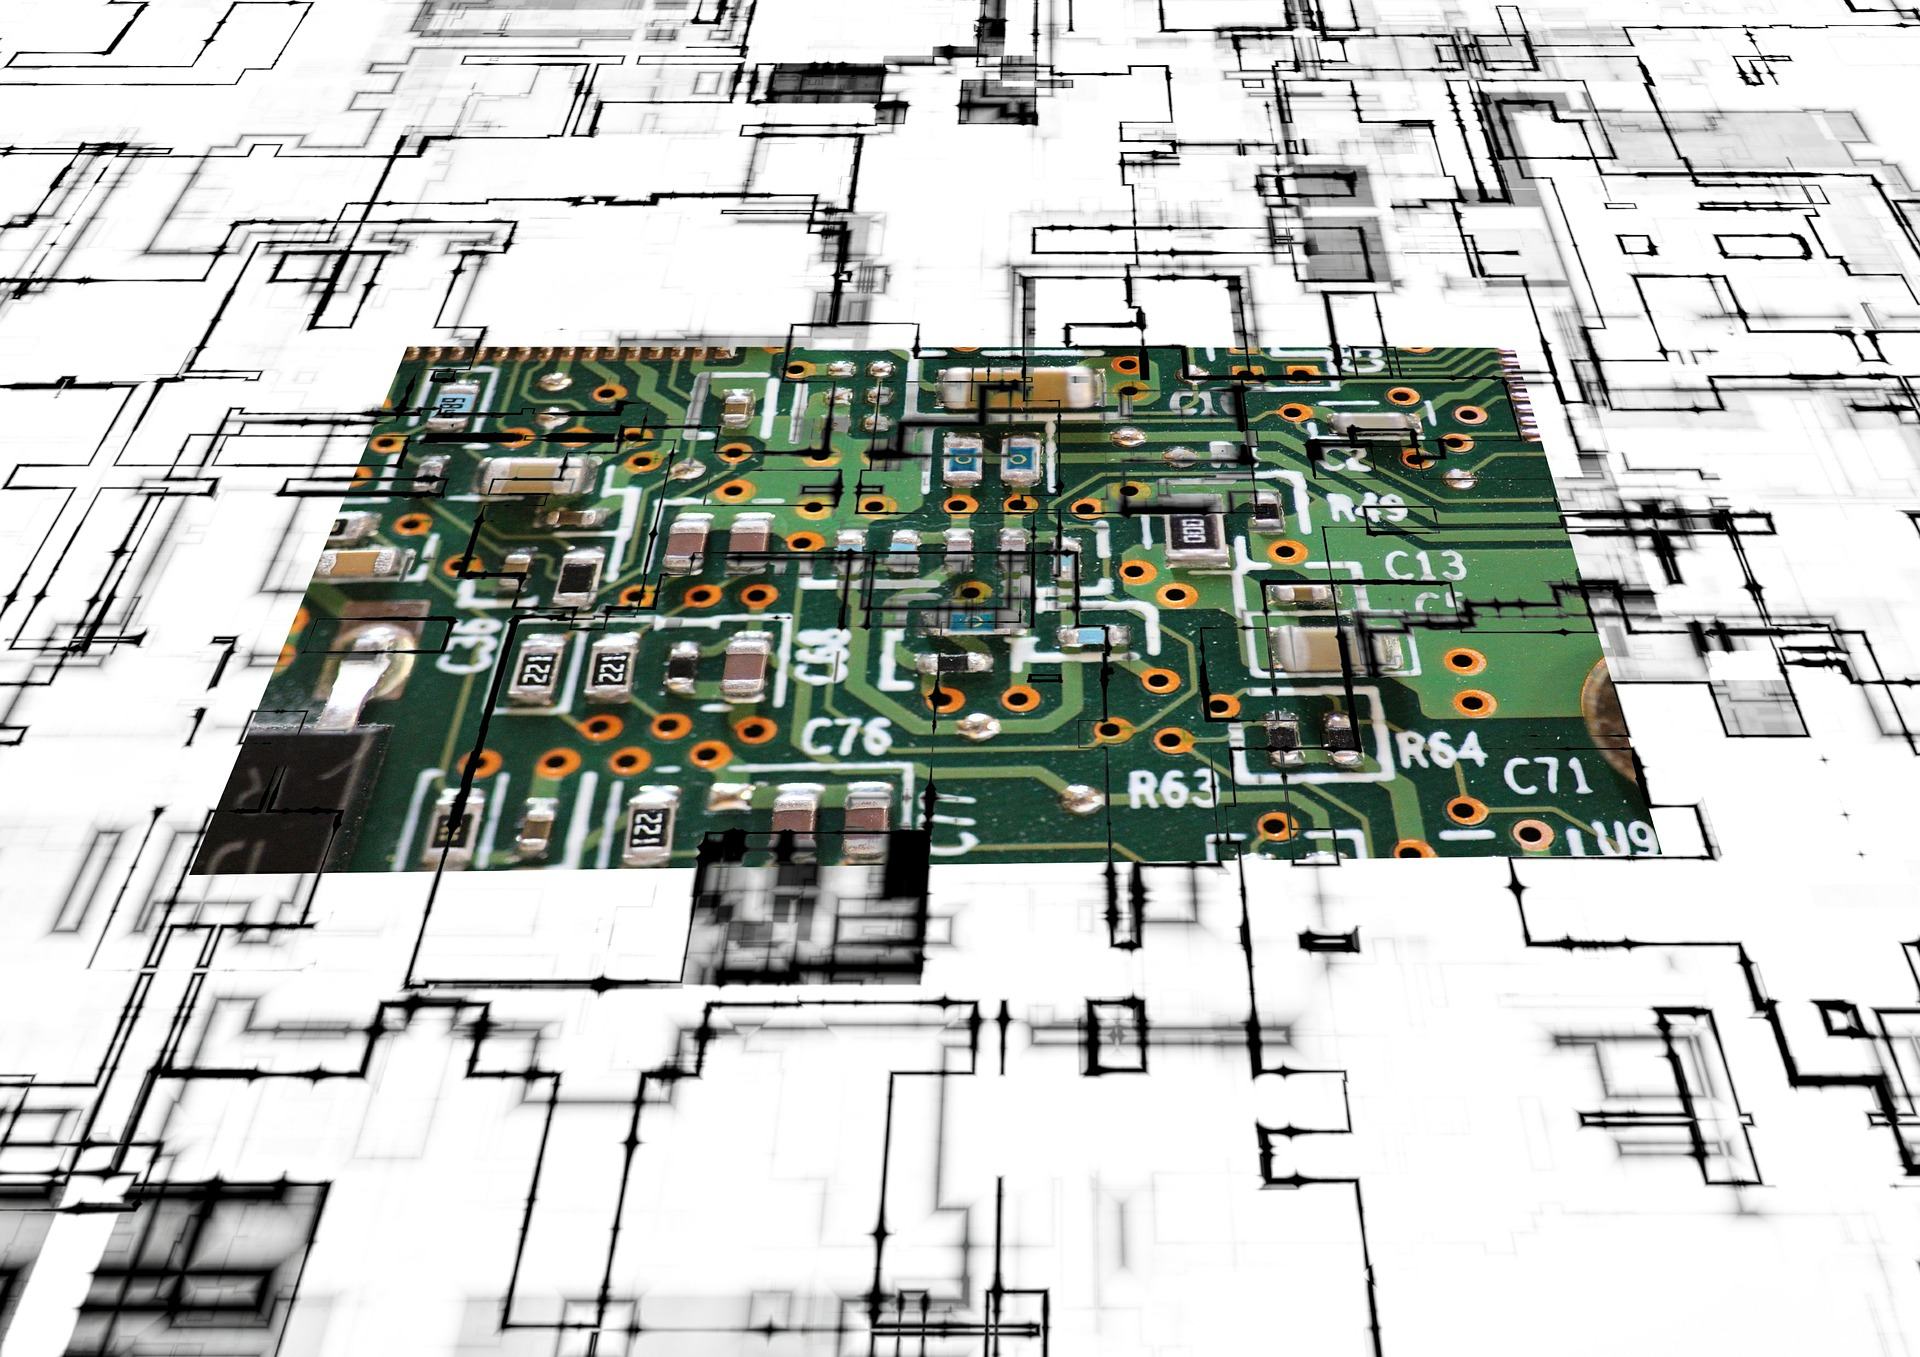
\includegraphics[width=\linewidth, trim={0 7cm 0 7cm}, clip]{board-410099_1920.jpg}}
% title graphic logo
\newcommand{\insertLogos}
{\centering 
\includegraphics[height=1.15cm]{logo.jpg}\hspace{1em}
\includegraphics[height=1.15cm]{Institute.jpg}}
%
% Title page of presentation
%
\makeatletter
\setbeamertemplate{title page}
{
	\vbox{}
	%
	\begin{center}
		\begin{minipage}[c]{0.8\linewidth}
			 
			\inserttitlegraphic
			    
			\begin{beamercolorbox}[sep=8pt,center]{title}
				\usebeamerfont{title}
				\inserttitle%
			\end{beamercolorbox}
			%
			\vspace{-2ex}\
			\begin{beamercolorbox}[sep=8pt,center]{author}
				\usebeamerfont{author}\small\insertauthor
				\vspace{3ex}
			\end{beamercolorbox}
			%
			\begin{minipage}[c]{.5\textwidth}
				\insertLogos
			\end{minipage}
			%
			\begin{minipage}[c]{.5\textwidth}
				\small
				\insertinstitute
			\end{minipage}%
			%
		\end{minipage}
	\end{center}
}
\makeatother
%
% start of document
%------------------------------------------------------------------------------
\begin{document}
%
% Title page
\begin{frame}[plain]
	\titlepage\cite{latex_bearmer_template}
\end{frame}
%
% \begin{frame}{Contents}
% 	\tableofcontents
% \end{frame}
%
%
\section{Introduction}
\begin{frame}{Intro}
	%
	\begin{block}{Call Graph} 
		Program Analysis, Inter-procedural Analysis,
	 	and Vulnerability Propagation Analysis.
	\end{block}

	\vfill
	%
    \begin{displayquote}{Contributions}
	\begin{itemize}
		\item Static approach for pragmatic call graph generation in Python.
		\item Micro-benchmark suite used as a standard to evaluate this methods in Python.
		\item Evaluating the effectiveness of the approach through Micro-benchmark and Macro-benchmarks 
		\item How the approach can aid dependency impact analysis through a potential enhancement of GitHub’s
		"security advisory"
	\end{itemize}
    \end{displayquote}
	%
\end{frame}
%
\section{Background}
%
\subsection{Challenges}
\begin{frame}{Challenges List}
	\begin{alertblock}{Python Features}
		\begin{itemize}
			\item Higher-order Functions
			\item Nested Definitions
			\item Classes
				\begin{itemize}
					\item Inherit attributes and methods
					\item Method Resolution Order (MRO)
				\end{itemize}
			\item Modules
			\item Dynamic Features 
				\begin{itemize}
					\item Meta-programming
				\end{itemize}
			\item Duck Typing
		\end{itemize}
	\end{alertblock}	
\end{frame}
%
\subsection{Limitations of Existing Static Approaches}
%
\begin{frame}{\textit{crypto} module}
	\begin{center}
		\lstinputlisting[language=python,title=crypto.py]{Code/crypto.py}\label{code:crypto}	
	\end{center}
	\footnote{Jump to Scope Tree(Figure.\ref{fig:scope_tree}), Assignment Graph(Page \ref{fig:assign})}
\end{frame}
%
\begin{frame}{Call graphs for \textit{crypto} module}
	\begin{figure}[htp]
		\begin{columns}[totalwidth=\linewidth]
			\begin{column}{0.3\columnwidth}
				\begin{subfigure}
					\centering
					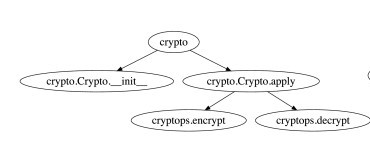
\includegraphics[width=0.33\paperwidth,height=0.33\paperheight]{call_graph_compare_a.jpg}
					\caption{Precise call graph.}
					\label{subfig:call_graph_compare_a}
				\end{subfigure}
			\end{column}
			\begin{column}{0.3\columnwidth}
				\begin{subfigure}
					\centering
					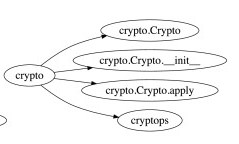
\includegraphics[width=0.33\paperwidth,height=0.33\paperheight]{call_graph_compare_b.jpg}
					\caption{Pyan-generated call graph}
					\label{subfig:call_graph_compare_b}
				\end{subfigure}
			\end{column}
			\begin{column}{0.3\columnwidth}
				\begin{subfigure}
					\centering
					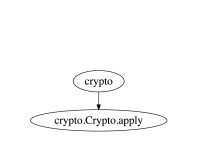
\includegraphics[height=0.33\paperheight]{call_graph_compare_c.jpg}
					\caption{Depends-generated call graph.}
					\label{subfig:call_graph_compare_c}
				\end{subfigure}
			\end{column}
		\end{columns}	
	\label{fig:call_graph_compare}	
	\end{figure}	
\end{frame}
%
\section{Topic}
%
\subsection{The Core Analysis}
%

%
\subsubsection{Syntax}
\begin{frame}{Syntax Analysis -- AST}
	%
	\begin{figure}
		\centering
		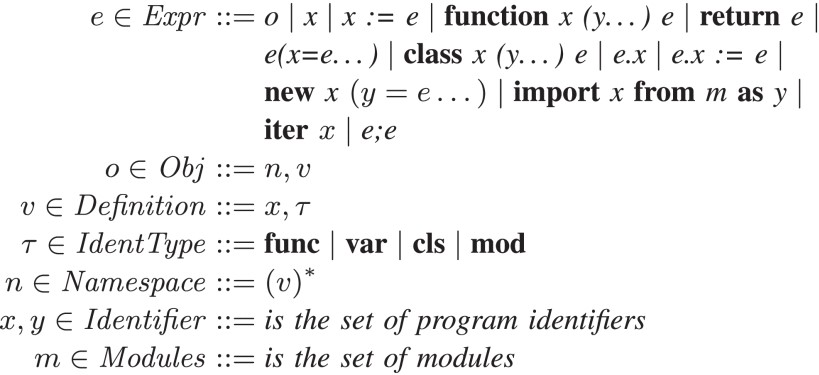
\includegraphics[height=0.5\paperheight]{AST.png}
		\caption{The syntax for representing the input Python programs along with the evaluation contexts}
		\label{fig:ast}
	\end{figure}		
	%
	\footnote{Jump to Scope Tree(Figure.\ref{fig:scope_tree}), Assignment Graph(Page \ref{fig:assign})}
\end{frame}

\begin{frame}{Syntax Analysis -- Evaluation}
	%
	\begin{block}{Evaluation $E$}
		Use evaluation contexts \cite{felleisen2009semantics}, \cite{madsen2017model} that describe the order in which sub-expressions are evaluated.
	\end{block}
	\begin{align*}
		E ::= & \left[ \right]|x:= E|\text{return} \; E|E(x=e\ldots)| \\
			  & o(x=E\ldots)| \text{new}\; x(y=E)| E.x | E.x:=e| \\
			  & o.x:=E|\text{iter}\; o |E;e|o;E
	\end{align*}		
	%
\end{frame}
%
\subsubsection{State}
\begin{frame}{State Analysis}
	%
	\vfill
	After the AST (Figure.\ref{fig:ast}), the analysis maintains a state consisting of four domains as shown:

	\begin{align*}
		\pi &\in AssignG =  Obj \hookrightarrow P(Obj) \\
		s &\in Scope = Definition \hookrightarrow P(Definition) \\
		h &\in ClassHier = Obj \hookrightarrow Obj^{*} \\
		\sigma &\in State = AssignG \times Scope \times Namespace \times ClassHier
	\end{align*}
	\footnote{Jump to AST(Figure.\ref{fig:ast})}
\end{frame}
%
%
\begin{frame}{Scope Tree}\label{frame:scope_tree}
	\begin{figure}
		\centering
		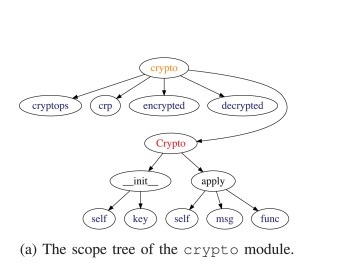
\includegraphics[height=0.5\paperheight]{scope_tree.jpg}
		\caption{The scope tree of the \textit{crypto} module}
		\label{fig:scope_tree}
	\end{figure} 
	\footnote{Return to Code demo(Page \ref{code:crypto}), AST(Figure.\ref{fig:ast})}
\end{frame}

\begin{frame}{Assignment Graph}\label{frame:assign_graph}
	\begin{figure}
		\centering
		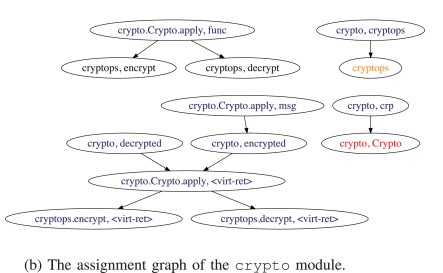
\includegraphics[height=0.5\paperheight]{assign_graph.jpg}
		\caption{The assignment graph of the \textit{crypto} module}
		\label{fig:assign}
	\end{figure} 
	\footnote{Return to Code demo(Page \ref{code:crypto}),  AST(Figure.\ref{fig:ast})}
\end{frame}
%
\subsubsection{Analysis Rules}
\begin{frame}{Analysis Rules}
	Demonstrating the state transition rules of analysis, the rules follow the form:
	\begin{equation}
		\left\langle \pi, s, n, h, E\left[e\right] \right\rangle \rightarrow \left\langle \pi^{'},  s^{'}, n^{'}, h^{'}, E\left[e^{'}\right] \right\rangle 
	\end{equation}\label{equ:state}
	When having an expression $e$ in the evaluation context $E$
	\begin{equation}
		\text{E-CTX} : \frac{\left\langle \pi, s, n, h, E\left[e\right] \right\rangle \hookrightarrow \left\langle \pi^{'},  s^{'}, n^{'}, h^{'}, e^{'} \right\rangle}
		{\left\langle \pi, s, n, h, E\left[e\right] \right\rangle \rightarrow \left\langle \pi^{'},  s^{'}, n^{'}, h^{'}, E\left[e^{'}\right] \right\rangle }
	\end{equation}\label{equ:E-CTX}
	\vfill
	%
	\begin{block}{\textit{getObject(s, n, x)}}
		The function iterates every element $y$ of the namespace $n$ in the reverse order, checking whether the element node y has
		any child matching the identifier $x$
	\end{block}
	%
	\begin{exampleblock}{\textit{addScope(s, n, x, t)}}
		This function adds an edge from the node accessed by the path $n$ to the target node given by
		the definition ($x$ ,$t$ )
	\end{exampleblock}
	%
	\begin{alertblock}{\textit{getClassAttrObject(o, x, h)}}
		This function deals with multiple inheritance, retrieving the object corresponding
		to the attribute $x$ of the receiver object $o$, the analysis by examining the hierarchy of classes $h$ 	
	\end{alertblock}
	%
\end{frame}
%
\begin{frame}{Python Source Code}
	\begin{columns}[totalwidth=\linewidth]
		\begin{column}{0.5\columnwidth}
			%
			\begin{center}
				\lstinputlisting[language=python,title=main.py]{Code/main.py}
			\end{center}
			%
		\end{column}
		\begin{column}{0.5\columnwidth}
			\begin{center}
				\lstinputlisting[language=python,title=main.py]{Code/test2.py}
			\end{center}
		\end{column}
	\end{columns}
\end{frame}
%
\begin{frame}{Analysis Rules}
	\begin{figure}[htp]
		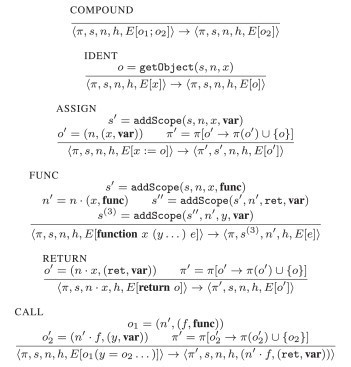
\includegraphics[height=0.75\paperheight]{analysis_rule_1.jpg}
		\caption{Rules of the analysis (1)}
		\label{fig:analysis_rule_1}
	\end{figure}
\end{frame}
%
\begin{frame}{Analysis Rules}
	\begin{figure}[htp]
		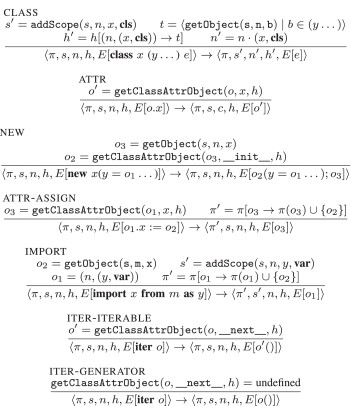
\includegraphics[height=0.75\paperheight]{analysis_rule_2.jpg}
		\caption{Rules of the analysis (2)}
		\label{fig:analysis_rule_2}
	\end{figure}
\end{frame}
%
\subsection{Call Graph Construction}
%
\begin{frame}
	\begin{alertblock}{Producing a call graph:}
		\begin{equation}
		cg \in CallGraph = Obj \hookrightarrow P(Obj)
		\end{equation}	\label{equ:cg}
	\end{alertblock}
	
	\vfill
	Algorithm (Figure.\ref{fig:algo}) takes two elements as input: 
	\begin{enumerate}
		\item a program $p \in Program$ of the model language whose syntax is
shown in Figure.\ref{fig:ast}.
		\item the final state $\sigma \in State$ stemming from the analysis step.
	\end{enumerate}
	
	
\end{frame}
%
\begin{frame}{Algorithm}
	\begin{figure}[htp]
		\centering
		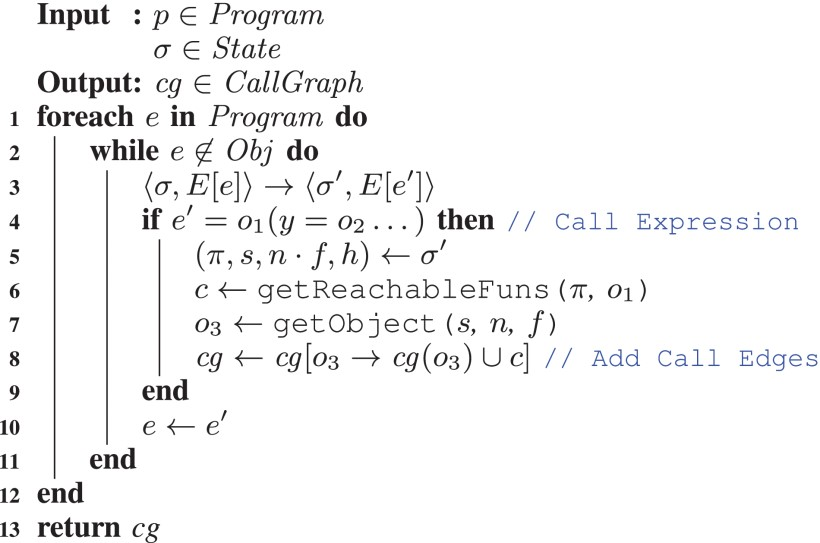
\includegraphics[width=\textwidth,height=0.75\paperheight]{algo.jpg}
		\caption{Algorithm for call graph construction.}
		\label{fig:algo}
	\end{figure}
\end{frame}
%
\section{Evaluation and Implementation} 
%
\begin{frame}{Outlook}
	
	Evaluating the approach based on three research questions:
	\begin{exampleblock}{}
		\begin{itemize}
			\item[RQ1] Is the proposed approach effective in constructing call
			graphs for Python programs?
			\item[RQ2] How does the proposed approach stand in comparison
			with existing open-source, static-based approaches for
			Python? 
			\item[RQ3] What is the performance of our approach?
		\end{itemize}
	\end{exampleblock}
\end{frame}

\begin{frame}{Setup}
	\begin{alertblock}{Experiments on a \textbf{Debian 9 host} with 16 CPUs and 16 GBs of RAM.}			
		\begin{enumerate}
			\item a micro-benchmark suite containing 112 minimal Python programs.
			\item a macro-benchmark suite of five popular real-world Python packages.	
		\end{enumerate}
	\end{alertblock}

\end{frame}
% 
%
\subsection{Micro-benchmark}
%
\begin{frame}{Micro-benchmark}
	\begin{figure}[htp]
		\centering
		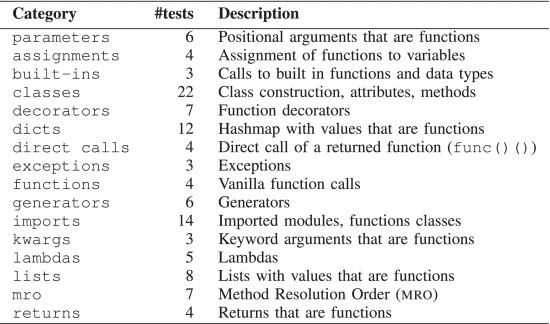
\includegraphics[width=\textwidth,height=0.6\paperheight]{Micro-Benchmark.jpg}
		\caption{Micro-benchmark for the suite categories.}
		\label{fig:micro_benchmark}
	\end{figure}
	
\end{frame}
%
\begin{frame}{Addressing Validity Threats}
	
	Asking two Python developers to rank the suite (from 1 to 10) based on the following criteria:
	\begin{exampleblock}{}
		\begin{enumerate}
			\item Completeness : Does it cover Python features?
			\item Code Quality : Are the tests unique and minimal?
			\item Description : Does the description adequately describe the given test case?
		\end{enumerate}
	\end{exampleblock}
\end{frame}
%
\begin{frame}{Micro-benchmark Suite Results}
	\begin{figure}[htp]
		\centering
		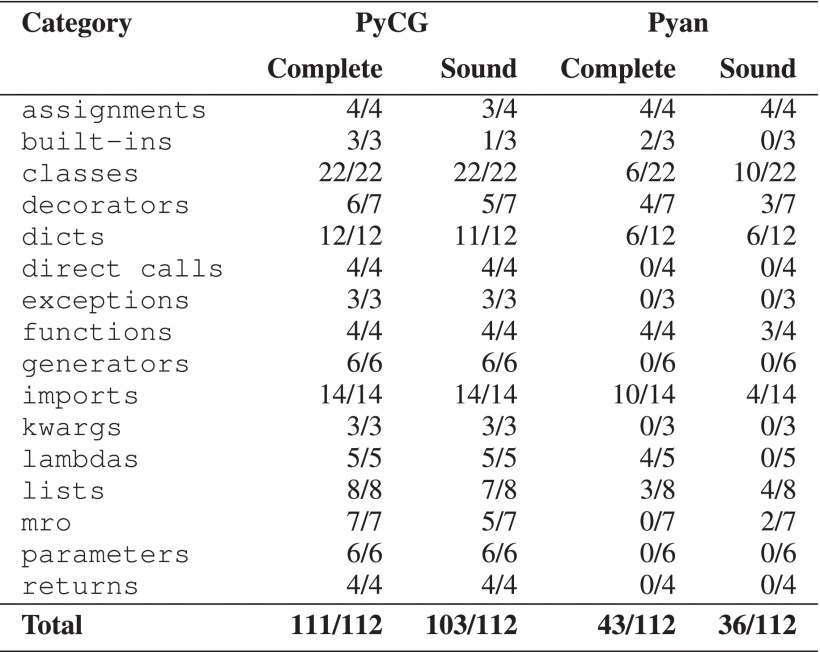
\includegraphics[width=0.8\textwidth,height=0.6\paperheight]{Micro-Benchmark_Results.jpg}
		\caption{Micro-benchmark results for PyCG and Pyan.
		Depends is unsound in all cases and complete in 110/112 cases
		and is omitted.}
		\label{fig:micro_benchmark_results}
	\end{figure}
\end{frame}
%
\subsection{Macro-benchmark}
\begin{frame}{Macro-benchmark}
	\begin{figure}[htp]
		\centering
		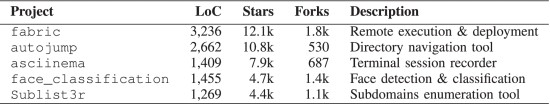
\includegraphics[width=\textwidth,height=0.65\paperheight]{Macro-Benchmark.jpg}
		\caption{Macro-benchmark suite project details.}
		\label{fig:macro_benchmark}
	\end{figure}
\end{frame}
%
\begin{frame}{Macro-benchmark Results}
	%
	\begin{figure}
		\centering
		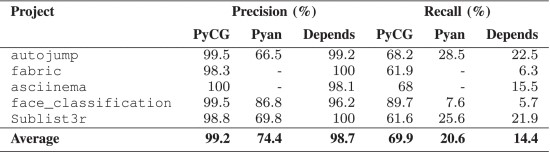
\includegraphics[width=\textwidth,height=0.65\paperheight]{Macro-Benchmark_Results.jpg}
		\caption{Macro-benchmark results and tool comparison.}
		\label{fig:macro_benchmark_results}
	\end{figure}
	%
\end{frame}
%
\subsection{Time and Memory Performance}
\begin{frame}{Time and Memory Performance}
	%
	\begin{block}{Command}
		\textbf{UNIX command} : \textit{time}, \textit{pmap} (average out of 20 runs)
	\end{block}
	\begin{figure}
		\centering
		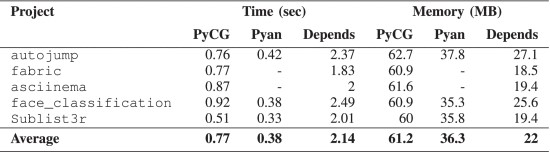
\includegraphics[width=\textwidth,height=0.5\paperheight]{Time-Memory-Performance.jpg}
		\caption{Time and Memory Performance.}
		\label{fig:Time-Memory-Performance}
	\end{figure}
	%
\end{frame}
%
\subsection{Case Study}
\begin{frame}{Case Study: A Fine-grained Tracking of Vulnerable Dependencies}
	%
	Further, we show a potential application through the enhancement
of GitHub's "security advisory"\cite{Advisory_Database} notification service.

\begin{alertblock}{Cases contained functional vulerability}
	\begin{enumerate}
		\item \textbf{PyYAML}\cite{PyYaml}  (versions before 5.1), a YAML parser affected by CVE-2017-18342 \cite{CVE-2017-18342}.
		\item \textbf{Paramiko}\cite{Paramiko}  (multiple versions before 2.4.1), an
		implementation of the SSHv2 protocol affected by CVE-2018-7750 \cite{CVE-2018-7750}.
	\end{enumerate}
\end{alertblock}

\begin{block}{Results}
	\begin{itemize}
		\item The vulnerable function in PyYAML(i.e., \textit{load}) was invoked by 42/106 projects.
		\item In Paramiko, method ( \textit{start\_server} ) was not utilized at all by any of the 
		76 projects. We also observed that 12 projects did not invoke any library coming from Paramiko.
	\end{itemize} 
\end{block}
	%
\end{frame}
%
%------------------------------------------------------------------------------
%
\section{References}
%
\begin{frame}
	\frametitle{References (1)}
	\textbf{Paper}\\
	\printbibliography[keyword=inf]
	\vfill
	%
	\textbf{Related Work and Additional Literature}
	\small
	\printbibliography[keyword=add]
\end{frame}
%
\begin{frame}{References (2)}
	\textbf{Website Sources}\\[2ex]
	\small Title page:
	\fullcite{latex_bearmer_template}
	\vspace{2ex}
	
	\printbibliography[keyword=web]
\end{frame}
%

%
\begin{frame}{}
	\usebeamerfont{AAA}
	\begin{center}
		\LARGE \textbf{Thank you for your attention}\\[2ex] 
		\small Please feel free to ask any questions
		\vspace{10ex}
		
		Contact:\\
		\Contactmail
	\end{center}
\end{frame}
%
%------------------------------------------------------------------------------
\end{document}